\documentclass[a4paper,12pt]{article} 

\usepackage[unicode, pdftex]{hyperref}

% новая команда \RNumb для вывода римских цифр
\newcommand{\RNumb}[1]{\uppercase\expandafter{\romannumeral #1\relax}}

%Добавляет возможность искать и копировать текст
\usepackage{cmap}

%Убирает пробел между названием таблицы/рисунка и самой таблицей/рисунком
\usepackage{caption}
\captionsetup[table]{skip= -0 cm}
\captionsetup[figure]{skip= -0 cm}

%Выравнивание названия таблиц по левому краю
%\usepackage[nooneline]{caption} 
%Размеры отступов 
\usepackage[left=20mm, top=20mm, right=20mm, bottom=20mm, footskip=10mm]{geometry}

%Рисунки
\usepackage{graphicx}
\usepackage{wrapfig} %обтекание элементов
\graphicspath{{graphs}{figures}}  % папки с картинками

%Русский язык в формулах
\usepackage{mathtext}

%  Русский язык
\usepackage[T2A]{fontenc}			
\usepackage[utf8]{inputenc}			
\usepackage[english,russian]{babel}	

%Красная строка для первого абзаца
\usepackage{indentfirst}

%Готические буквы
\usepackage{amssymb}

% Математика
\usepackage{amsmath,amsfonts,amssymb,amsthm,mathtools} 
\usepackage{wasysym}

%Цветные подписи в таблице
\usepackage[table,xcdraw]{xcolor}

%Сделать несколько рядов одним
\usepackage{multirow}

\usepackage{fancyhdr} % Колонтитулы
 	\pagestyle{fancy}
 	\renewcommand{\headrulewidth}{0.3mm}  % Толщина линейки, отчеркивающей верхний колонтитул
 	%\lfoot{Нижний левый}
 	%\rfoot{Нижний правый}
 	\rhead{Белостоцкий Артмемий, Б04-006}
 	%\chead{Верхний в центре}
 	\lhead{Лабораторная работа №5.1.2}
 	\renewcommand{\footrulewidth}{0.3mm}
 	\cfoot{\thepage} % По умолчанию здесь номер страницы
 	
 	
%\captionsetup[table]{
%  position=above,
%  justification=raggedright,
  %labelsep=newline, % <<< label and text on different lines
%  singlelinecheck=false % <<< raggadright also when the cap%tion is shorter
                        % than a single line
%}
 	
\begin{document} 

%Титульник 
\begin{titlepage}
	\begin{center}
		\large 	МИНИСТЕРСТВО ОБРАЗОВАНИЯ И НАУКИ РОССИЙСКОЙ ФЕДЕРАЦИИ\\
				МОСКОВСКИЙ ФИЗИКО-ТЕХНИЧЕСКИЙ ИНСТИТУТ \\
				(НАЦИОНАЛЬНЫЙ ИССЛЕДОВАТЕЛЬСКИЙ УНИВЕРСИТЕТ)\\ 
				ФИЗТЕХ-ШКОЛА ЭЛЕКТРОНИКИ, ФОТОНИКИ \\
				И МОЛЕКУЛЯРНОЙ ФИЗИКИ \\
		
		
		\vspace{4.0 cm}
		Лабораторная работа № 5.1.2 \\ 
		\LARGE \textbf{Исследование эффекта Комптона}
	\end{center}
	\vspace{3 cm} \large
	
	\begin{flushright}
		выполнил студент 3 курса \\
		{группы Б04-006}\\
		\textbf{Белостоцкий Артемий}\\
	\end{flushright}
	
	\vfill

	\begin{center}
	Долгопрудный, 2022 г.
	\end{center}
\end{titlepage}                                                                      

\section*{Аннотация}

В данной работе исследуется эффект Комптона -- рассеяния $\gamma$-квантов на частицах, масса покоя которых рассчитывается из экспериментальных данных.

\section*{Теоретические сведения}

Эффектом Комптона называют изменение длины волны электромагнитного излучения при рассеянии. Впервые этот эффект наблюдался Комптоном (1923 г.) при рассеянии рентгеновских лучей.

Приведем расчет эффекта Комптона квантов рентгеновского излучения на неподвижных частицах массой $m$.

\begin{figure}[h!]
	\centering
	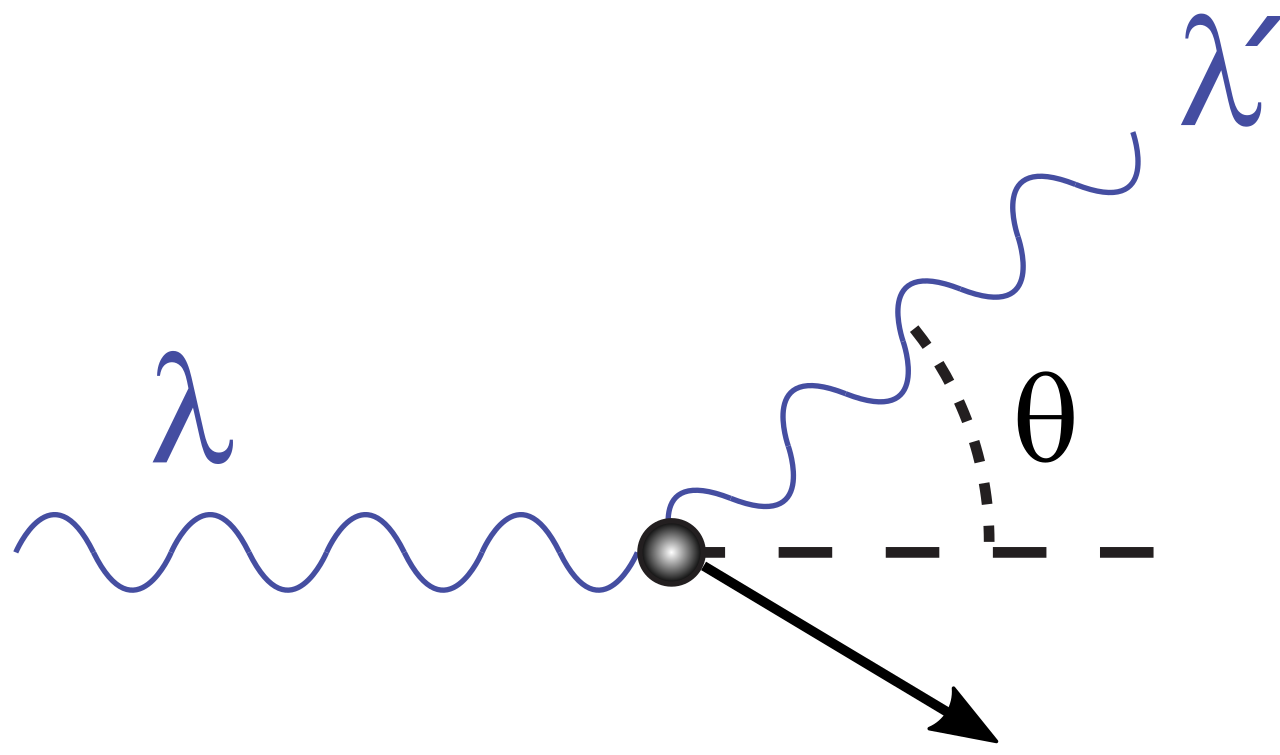
\includegraphics[width=0.6\linewidth]{Compton_scattering}
	\caption{Графическая схема эффекта Комптона на неподвижной частице}
\end{figure}

Запишем закон сохранения 4-импульса:

\begin{align*}
	P^{\mu}_{\gamma} &= \begin{bmatrix}
						\frac{h\nu}{c} \\
						\frac{h\nu}{c} \\
						0 \\
					   \end{bmatrix} \\
%
	P^{\mu}_m &= \begin{bmatrix}
					\frac{mc^2}{c} \\
					0 \\
					0 \\
				\end{bmatrix} \\	
%
	P'^{\mu}_{\gamma} &= \begin{bmatrix}
					      \frac{h\nu'}{c} \\
					      \frac{h\nu'}{c} \cos \theta \\
					      \frac{h\nu'}{c} \sin \theta \\
						 \end{bmatrix} \\
%	
	P'^{\mu}_m 	&= \begin{bmatrix}
					       \frac{E}{c} \\
					       p'_x \\
					       p'_y \\
					\end{bmatrix} \\				 			   
	P^{\mu}_{\gamma} + P^{\mu}_m &= P'^{\mu}_{\gamma} + P'^{\mu}_m \\
%
	P^{\mu}_{\gamma} + P^{\mu}_m &- P'^{\mu}_{\gamma} =  P'^{\mu}_m \\
\end{align*}

Возведем обе части равенства в квадрат, учитывая что $(P'^{\mu}_m, P'^{\mu}_m) = m^2 c^4$

\pagebreak

Пропуская математические выкладки, получим:

\begin{align} \label{eq1:compton_scattering}
	mc^2 \left( \frac{1}{h\nu'(\theta)} - \frac{1}{h\nu} \right) = 1 - \cos \theta
\end{align}

\section*{Экспериментальная установка}

\begin{figure}[h!]
	\centering
	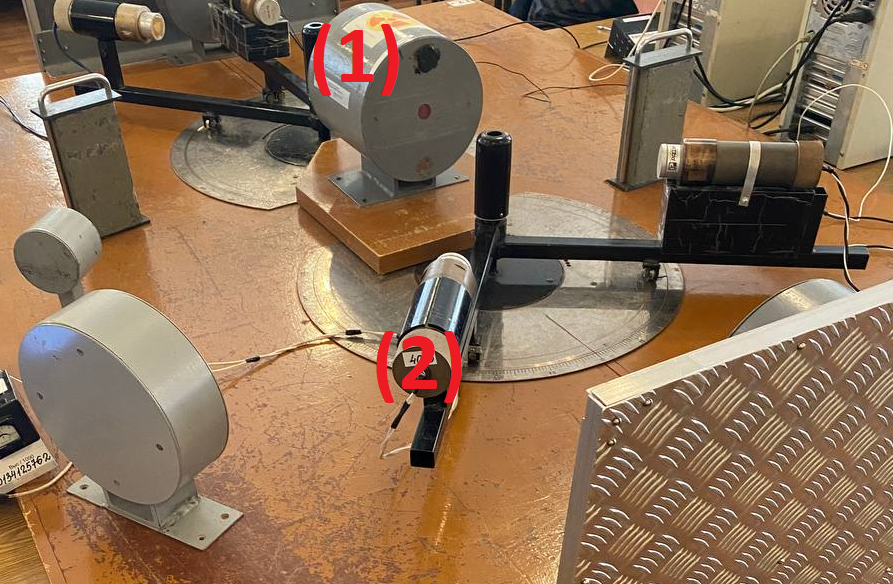
\includegraphics[width=0.8\linewidth]{setup_1}
	\caption{Экспериментальная схема. (1) -- источник $\gamma$-лучей, (2) -- ФУЭ}
\end{figure}

\begin{figure}[h!]
	\centering
	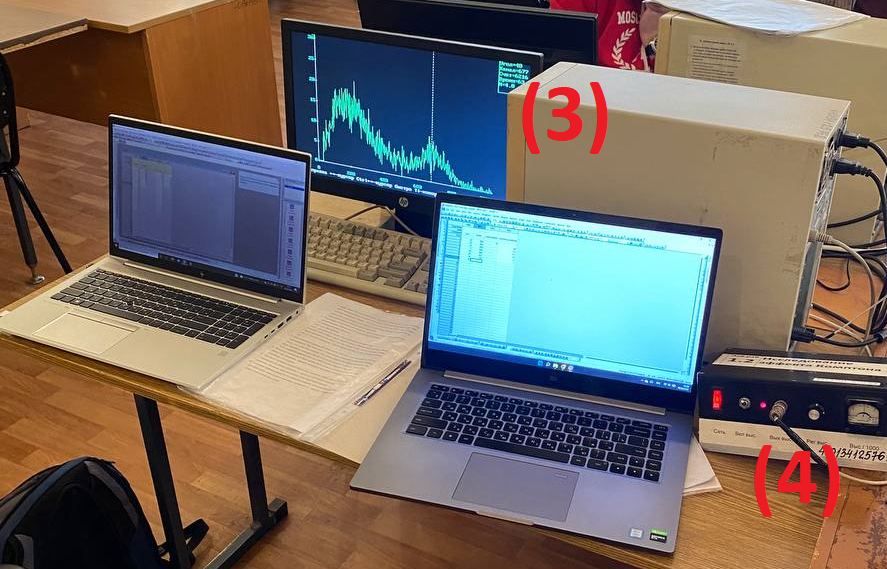
\includegraphics[width=0.8\linewidth]{setup_2}
	\caption{Экспериментальная схема. (3) -- компьютер, подключенный к ФЭУ, (4) -- блок управления ФЭУ}
\end{figure}

\pagebreak

\section*{Ход работы}

Так как энергия $\gamma$-кванта пропорциональна номеру в анализаторе, то формула (\ref{eq1:compton_scattering}) может быть представлена в виде:

\begin{align} \label{eq2:approxiamtion}
	\frac{1}{N(\theta)} = A + B (1 - \cos (\theta + \theta_0) ),
\end{align}

где $A, B, \theta_0$ -- некоторые константы. Добавка $\theta_0$ связана с неидеальной центровкой всей системы.

Снимем зависимость $N(\theta)$, построим соответствующий график и аппроксимируем соответствующей функцией, представленной выше:

\begin{figure}[h!]
	\centering
	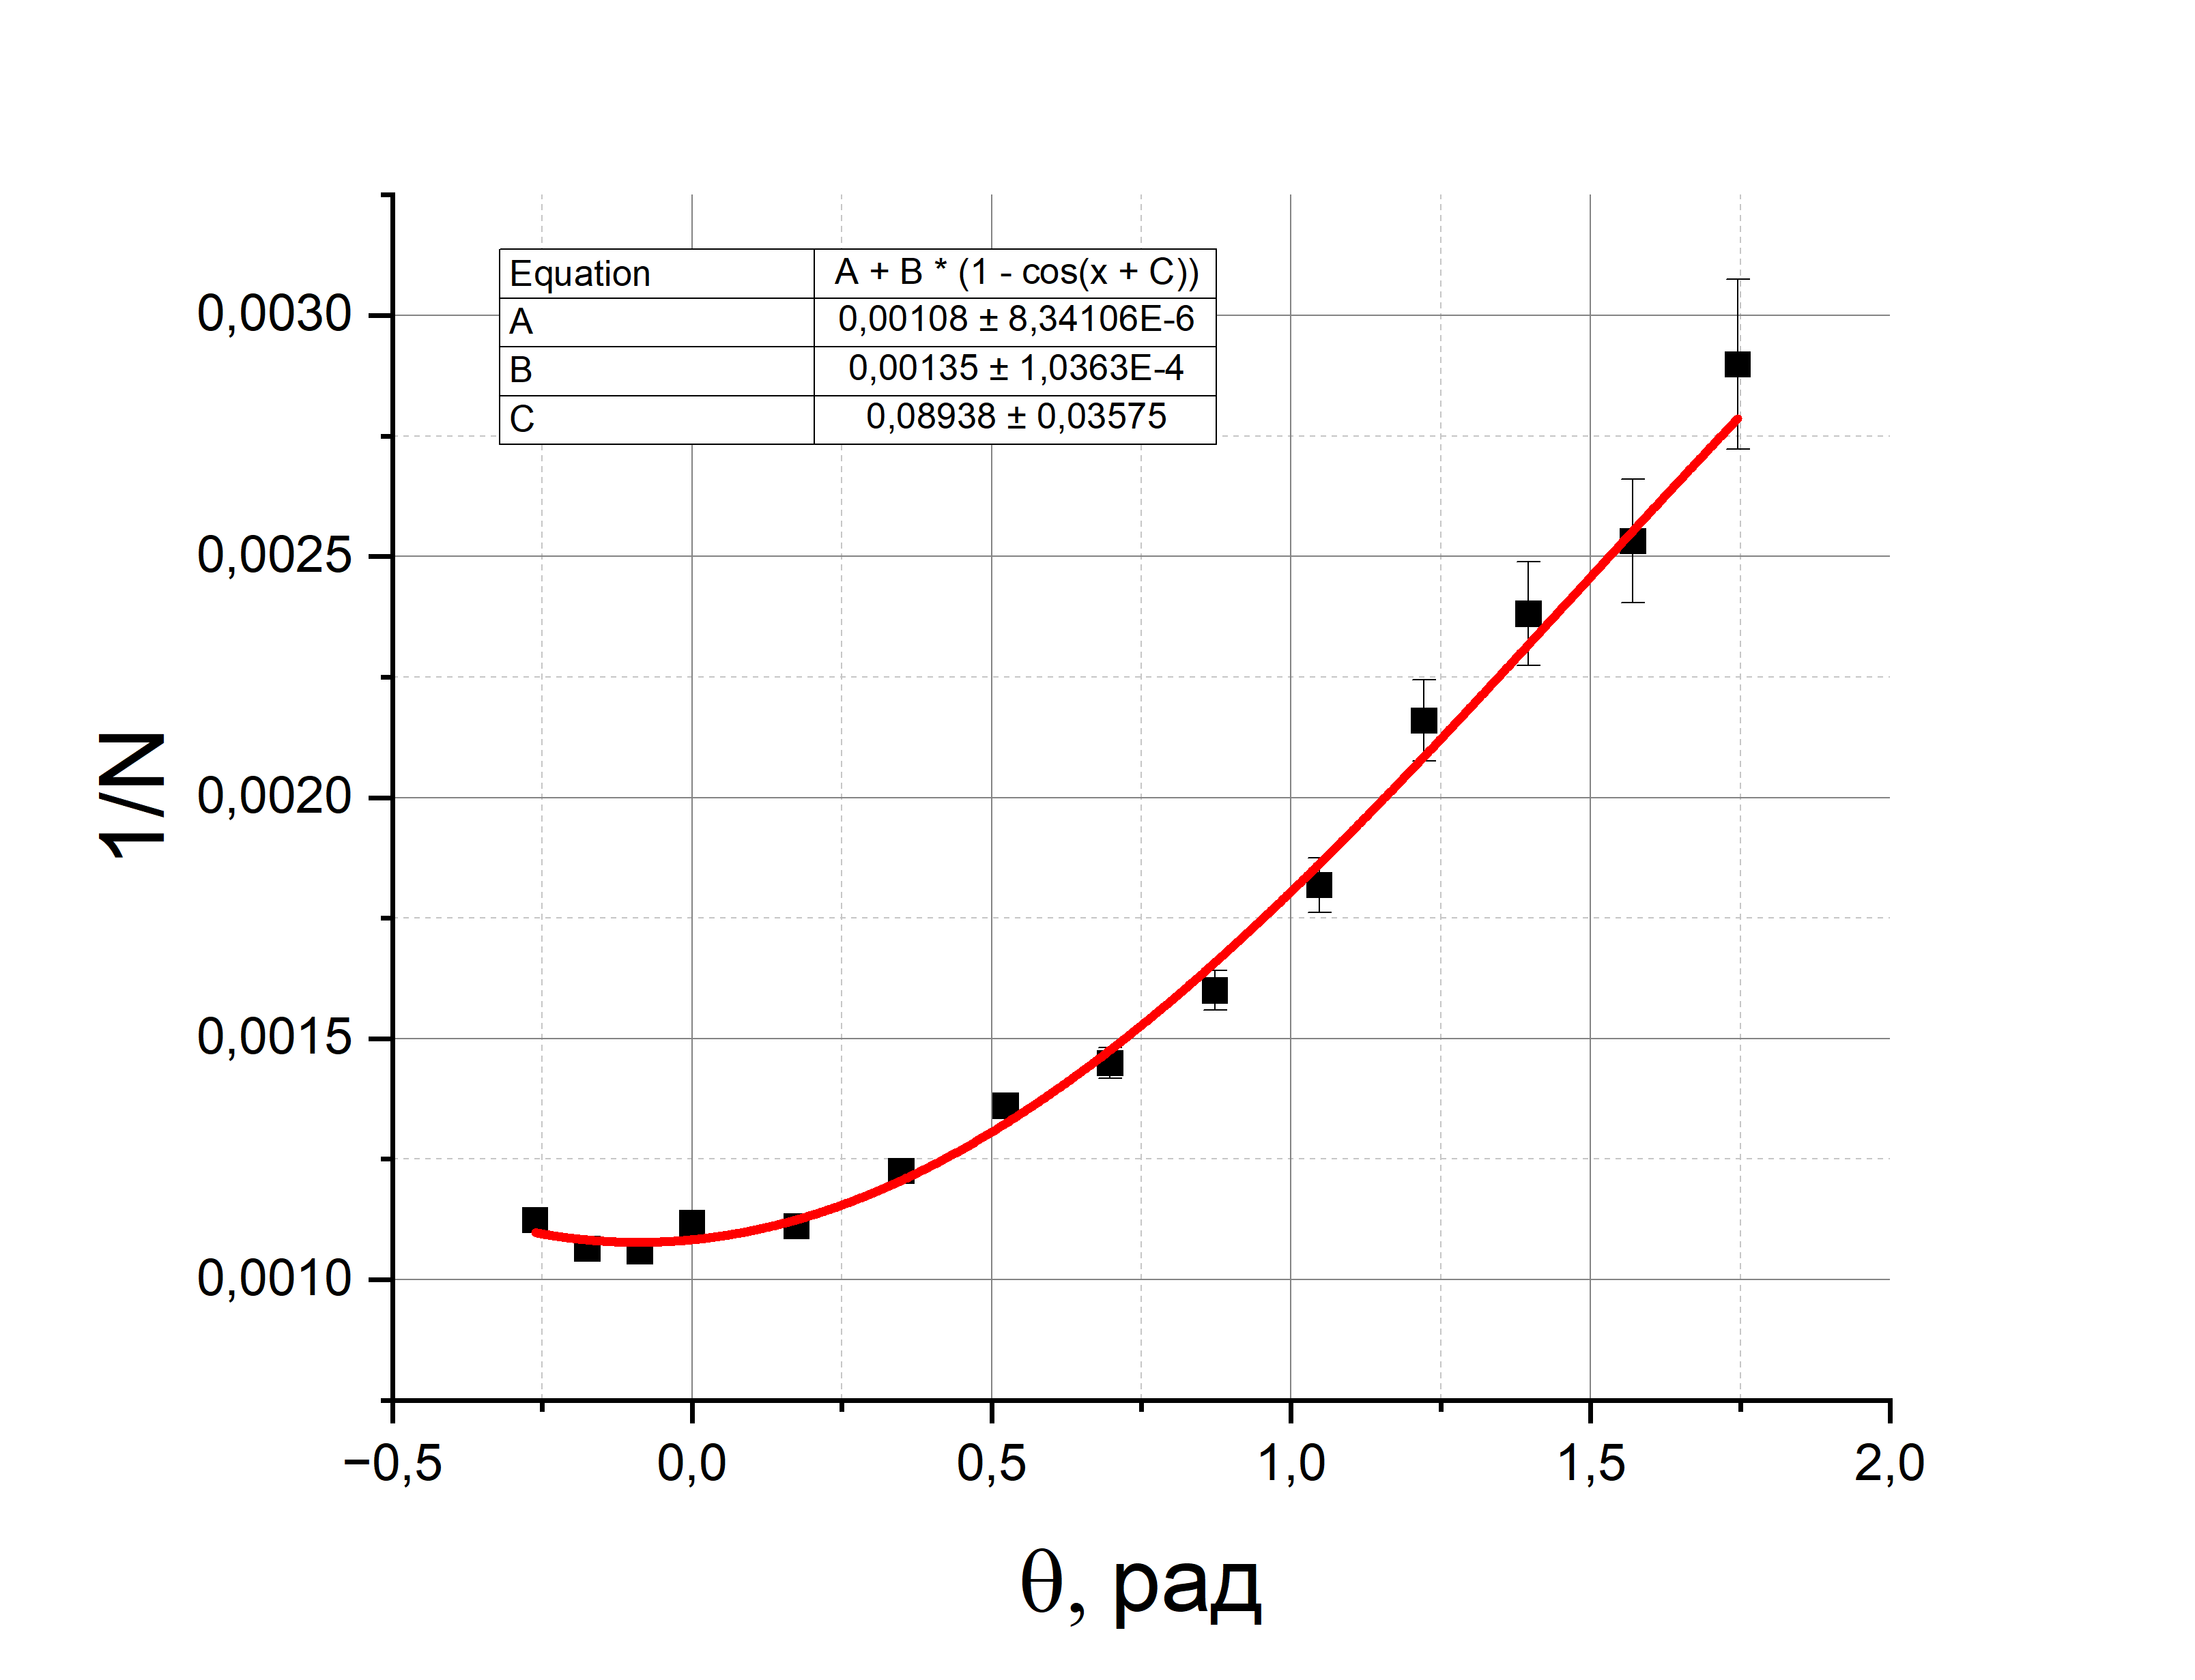
\includegraphics[width=\linewidth]{Chanel_num}
	\caption{Зависимость $N(\theta)$}
\end{figure}

Положим в формуле (\ref{eq2:approxiamtion}) $\theta = \frac{\pi}{10}$ и, учитывая что $N(\theta) \sim h\nu(\theta)$, найдем массу покоя частиц, на которых происходит рассеяние:

$$
	mc^2 = h\nu \frac{N(\frac{\pi}{10}) (1 - \cos (\frac{\pi}{10} + \theta_0) )}{N(0) - N(\frac{\pi}{10})},
$$

В нашем случае источником является $^{137}Cs$, тогда $h\nu = 662$ кэВ, тогда масса покоя:

$$
	mc^2 \approx (556 \pm  111) кэВ
$$ 

\pagebreak

\subsubsection*{Комптоновский край рассеяния}

Теоретическое значение для края комптоновского рассеяния:

$$
	E_к = \frac{h\nu}{1 + \frac{mc^2}{h\nu}}
$$

Найдем коэффициент пропорциональности между энергий и номером канала (для нулевого угла):

$$
	k = \frac{E(0)}{N(0)} = \frac{662}{895} \approx 0,74 \  кэВ
$$

Тогда, измерив по спектру номер канала, соответствующего краю комптоновского рассеяние ($N_к = 570$) можно также оценить массу покоя электрона:

$$
	mc^2 \approx 378 кэВ
$$

Расхождение с теоретическим значением может быть связано с неточным определением комптоновского края на спектре.

\section*{Выводы}

\begin{itemize}
	\item В ходе работы была получена масса покоя ($mc^2 = (556 \pm 111) кэВ)$ частицы (электрона), на которой происходит Комптоновское рассеяние, причем полученные данные хорошо соотносятся с теоретическими ($m_ec^2 = 511 кэВ$)
\end{itemize}

\newpage

\section*{Приложение}

В приложении приведем спектры полученные на лабораторном компьютере.

\begin{figure}[h!]
	\centering
	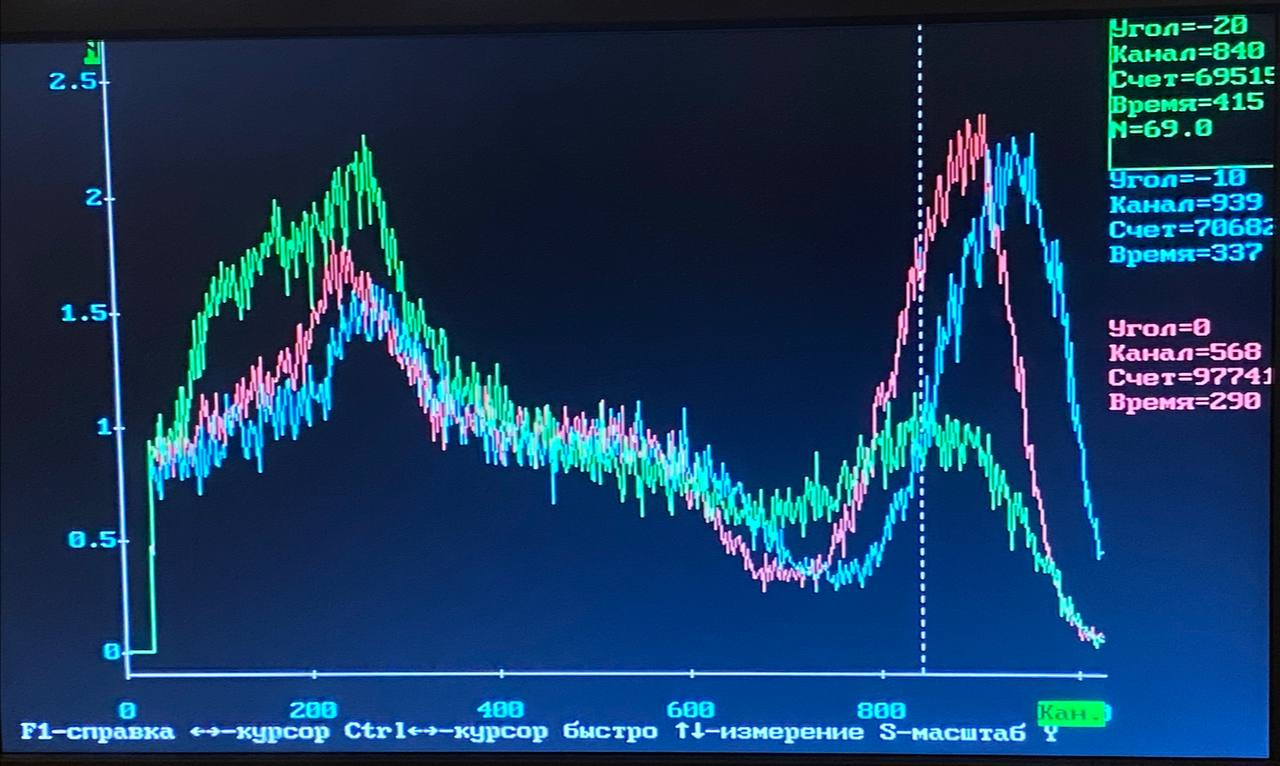
\includegraphics[width=0.8\linewidth]{spectre_1}
	\caption{Картина спектра $\gamma$-излучения, полученная на компьютере для различных углов рассеяния}
\end{figure}

\begin{figure}[h!]
	\centering
	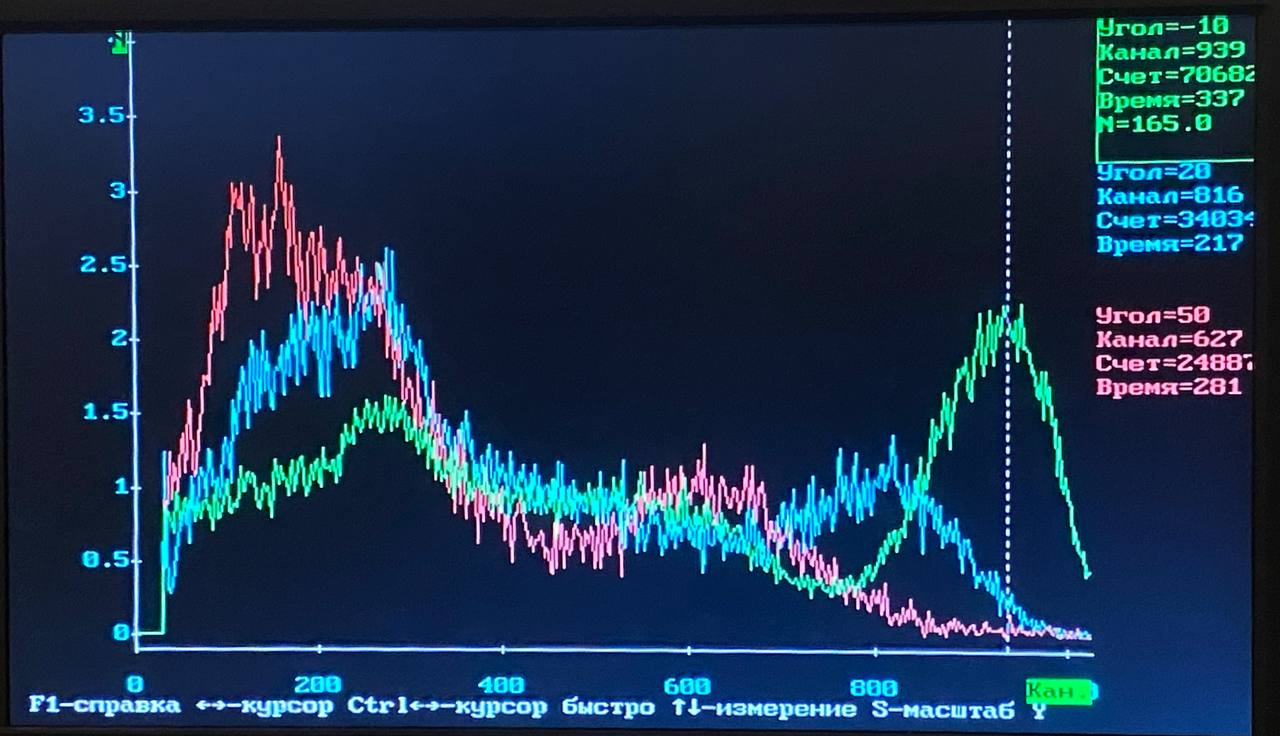
\includegraphics[width=0.8\linewidth]{spectre_2}
	\caption{Картина спектра $\gamma$-излучения, полученная на компьютере для различных углов рассеяния}
\end{figure}


\end{document}